\chapter{Application de démonstration}

\section{Objectifs}

Afin de présenter les fonctionnalités offertes par la bibliothèque, une application de démonstration a été développée. Initialement prévue comme une application d'organisation pour une équipe de jeu en ligne, les fonctionnalités ont été revues à la baisse lorsque le projet s'est orienté plus sur le développement d'une bibliothèque réutilisable.

Au final, l'application présente une version simplifiée de trois des modules initialement prévus, ce qui permet tout de même d'observer la bibliothèque en action et d'expérimenter les mises à jour en temps réel de l'interface en réponse aux interactions des autres utilisateurs du système.

\section{Modules}

	\subsection{Calendrier}
	\begin{figure}[h]
		\centering
		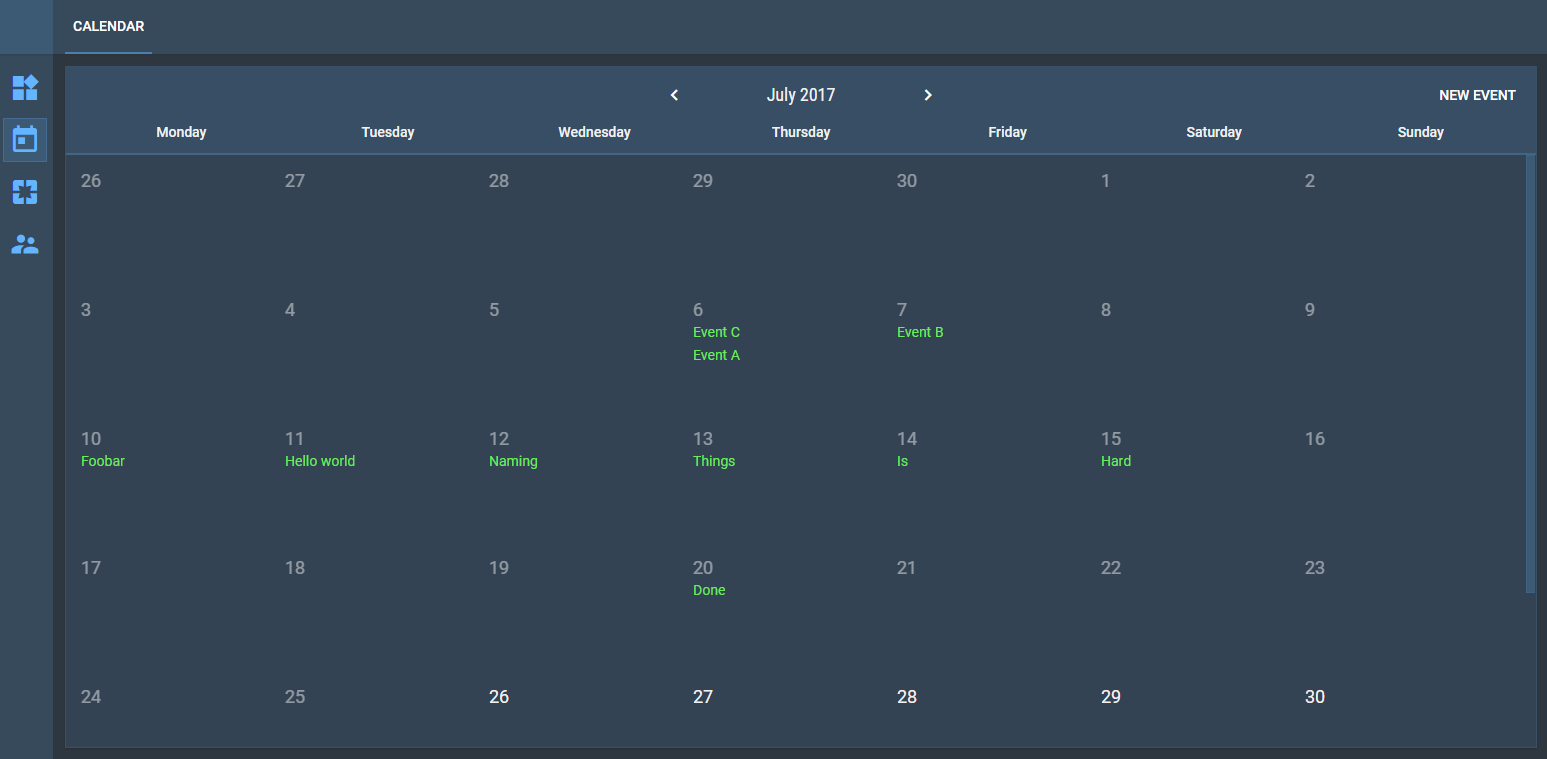
\includegraphics[width=12cm]{img/calendar}
		\caption{Module calendrier}
	\end{figure}
	
	Un système de calendrier dans lequel l'utilisateur peut saisir des événements qui seront visibles par tous les utilisateurs.
	
	\subsection{Composition de groupes}
	\begin{figure}[h]
		\centering
		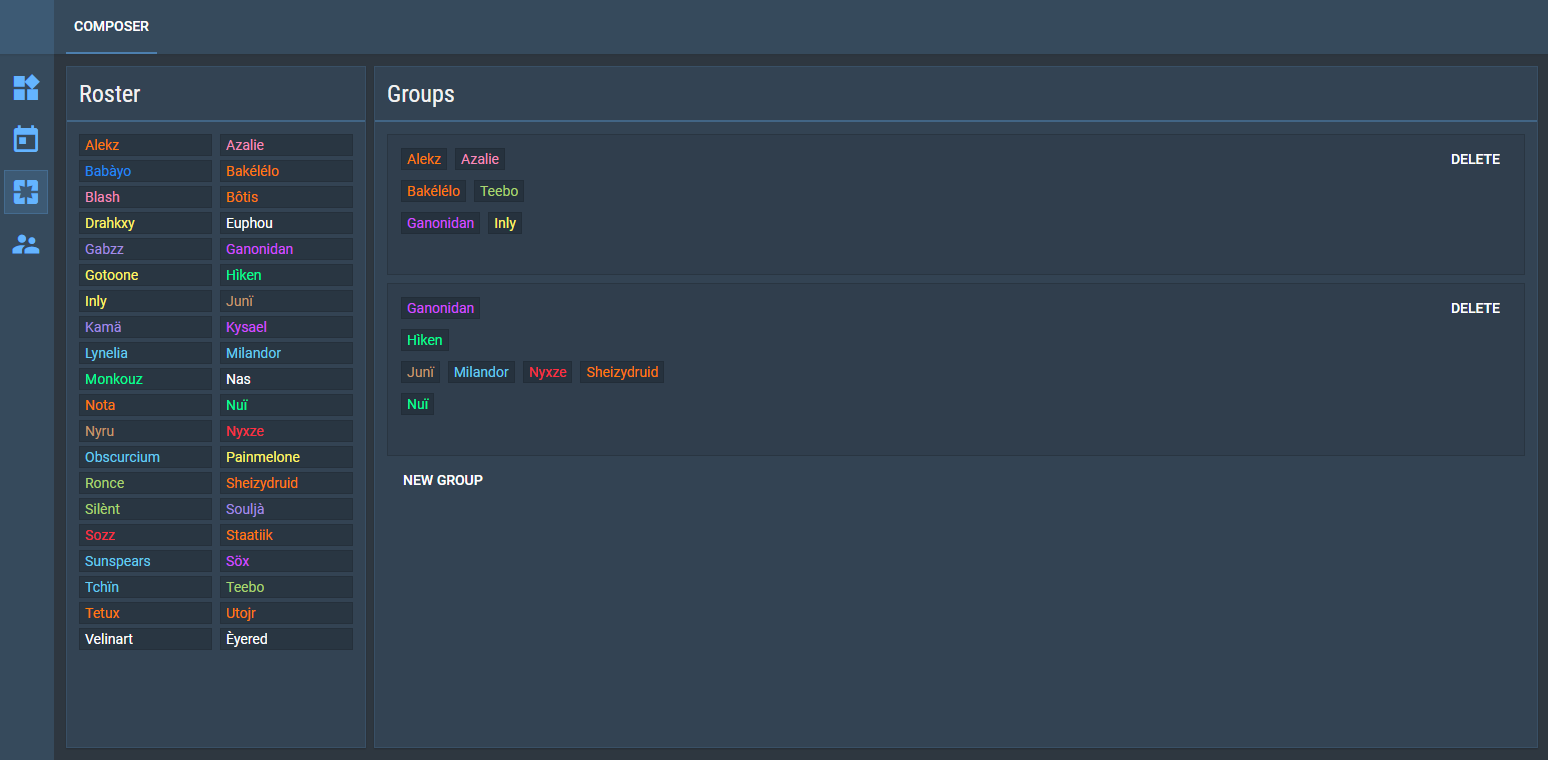
\includegraphics[width=12cm]{img/composer}
		\caption{Module composition de groupes}
	\end{figure}
	
	Un utilitaire de construction de groupes de jeu. Le panneau à gauche présente l'ensemble des joueurs enregistrés tandis que celui de droit permet de créer de groupes dans lesquels les joueurs pourront être placés.
	
	Chaque groupe est subdivisé en sous-groupes permettant d'organiser les joueurs au sein d'un même groupe. Un nouveau sous-groupe est créé dynamiquement lorsque tous les sous-groupes existants sont utilisés.
	
	Les joueurs peuvent être placés dans les groupes par \emph{drag-and-drop} entre les deux panneaux de l'interface.
	
	\subsection{Roster}
	\begin{figure}[h]
		\centering
		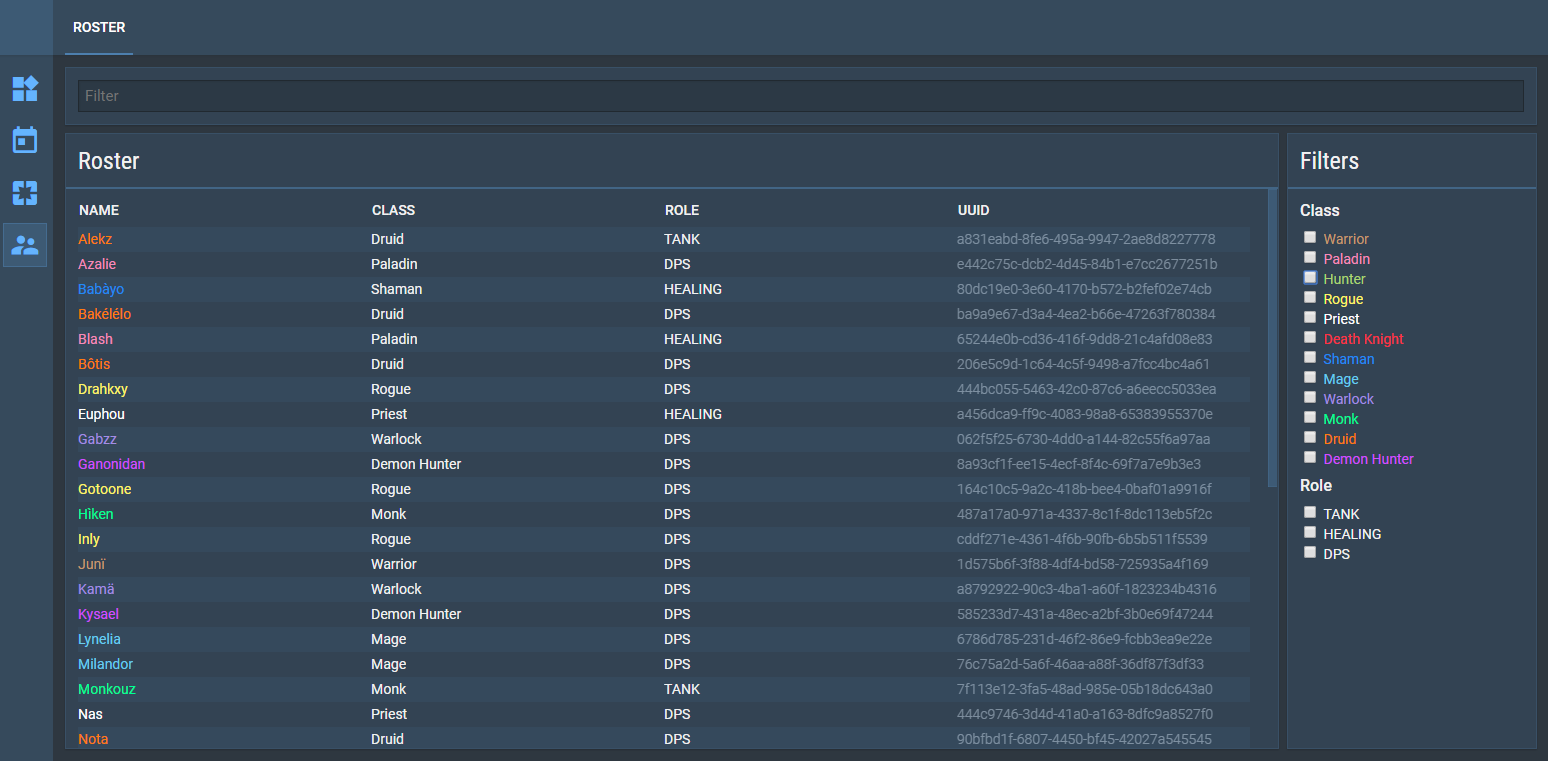
\includegraphics[width=12cm]{img/roster}
		\caption{Module \emph{roster}}
	\end{figure}
	
	Une vue d'ensemble des joueurs et de leur rôle. Une zone de recherche est disponible en haut de l'interface pour rechercher un utilisateur par nom. Les filtres sur le côté droite permettent de filtrer d'avantage la liste en fonction de la classe ou du rôle du joueur.
	
	Un clic doit sur le rôle d'un joueur ouvre un menu contextuel permettant de modifier le rôle du joueur.
	
\section{Implémentation}

	\subsection{Composants}
	
	L'application est construite sur la base de nombreux composants indépendant associés pour former l'interface complète.
	
	La racine de la structure est formée par les composants \texttt{GtRoot}, \texttt{GtTitlebar}, \texttt{GtSidebar} et \texttt{GtViewport}. Ceux-ci détermines le \texttt{layout} générale de l'interface et sont toujours présent à l'écran.
	
	L'élément \texttt{GtViewport} est utilisé comme élément hôte pour le \texttt{Router}. Celui-ci observe l'URL de la page courante et détermine le composant à afficher dans la zone principale de l'interface. Si aucune règle de routage définie ne correspond, l'utilisateur est redirigé sur la page du \emph{dashboard}.
	
	Si une règle correspond, le composant associé est instancié et inséré dans l'arbre DOM en tant qu'enfant de \texttt{GtViewport}. Les composants insérés de cette façon sont \texttt{GtCalendar}, \texttt{GtComposer} et \texttt{GtRoster}. Ceux-ci sont alors responsable de construire les niveaux inférieurs de la structure.
	
	\subsubsection{Composants communs}
	
	Un certain nombre de composants communs aux différents modules sont disponibles. Par exemple \texttt{GtBox} qui permet la construction des boîtes utilisée de façon extensive dans l'interface. Le composant \texttt{GtClassColor} permet de colorer automatiquement un texte avec la couleur d'une classe de joueur, celui-ci est principalement utilisé pour afficher le nom des joueurs de façon colorée.
	
	\subsection{Services}
	
	Les données sources utilisées pour générer l'interface sont gérée par trois implémentation de la classe \texttt{Service}: \texttt{CalendarService}, \texttt{ComposerService} et \texttt{ToonsService}. Ces services sont responsable de charger les données correspondantes depuis le serveur et de les exposer sous la forme de signaux au composants de l'application. Ils fournissent aussi les méthodes permettant de modifier ces données.
	
	\subsection{Communication client-serveur}
	
	L'application client utilise principalement une interface HTTP REST pour récupérer les données du serveurs et effectuer des modifications.
	
	Le mécanisme d'\texttt{EventSource}, introduit avec les \emph{Server-Sent Events}, est utilisé pour implémenter les notifications de mises à jour en temps-réel par le serveur. Une \texttt{EventSource} est un objet JavaScript utilisant une connexion HTTP \emph{chunked} pour recevoir les événements du serveur, ceux-ci sont alors émis en tant qu'événement DOM classique pouvant être écoutés avec la méthode habituelle \texttt{addEventListener} sur l'objet \texttt{EventSource}.
	
	Lorsqu'un service est activé, il récupère données les plus récentes depuis le serveur avec une requête HTTP \emph{GET}, il s'enregistre ensuite à l'\texttt{EventSource} afin de recevoir les notifications de mises à jour émises par le serveur et modifier ainsi sa base de données interne.
	